\newpage
\section{Proposed Credit Risk Prediction Model Based on Causal Machine Learning}
\noindent
This chapter presents in detail the methodology and the overall architecture of the credit risk prediction model based on Causal Machine Learning. We begin by establishing a specialised data processing pipeline that integrates techniques for class balancing (S\_Pro), feature selection (L\_Pro) and discretisation (K\_Pro) in order to construct an optimal sample space fully compatible with the probabilistic nature of the model. Next, the focus of the research turns to the core procedure that constitutes the Bayesian network (BN\_Pro), including the resolution of the optimisation problem in graph structure learning and the methods for estimating the parameter system. Finally, in order to affirm the system's capacity to make the financial decision flow transparent, we present the techniques for interpreting the results (In\_Pro), from sensitivity analysis and forward--backward inference to hypothetical intervention scenarios, while also establishing comprehensive criteria for evaluating predictive performance. The proposed model framework is described in Figure \ref{fig:framework}
\begin{figure}[H]
    \centering
    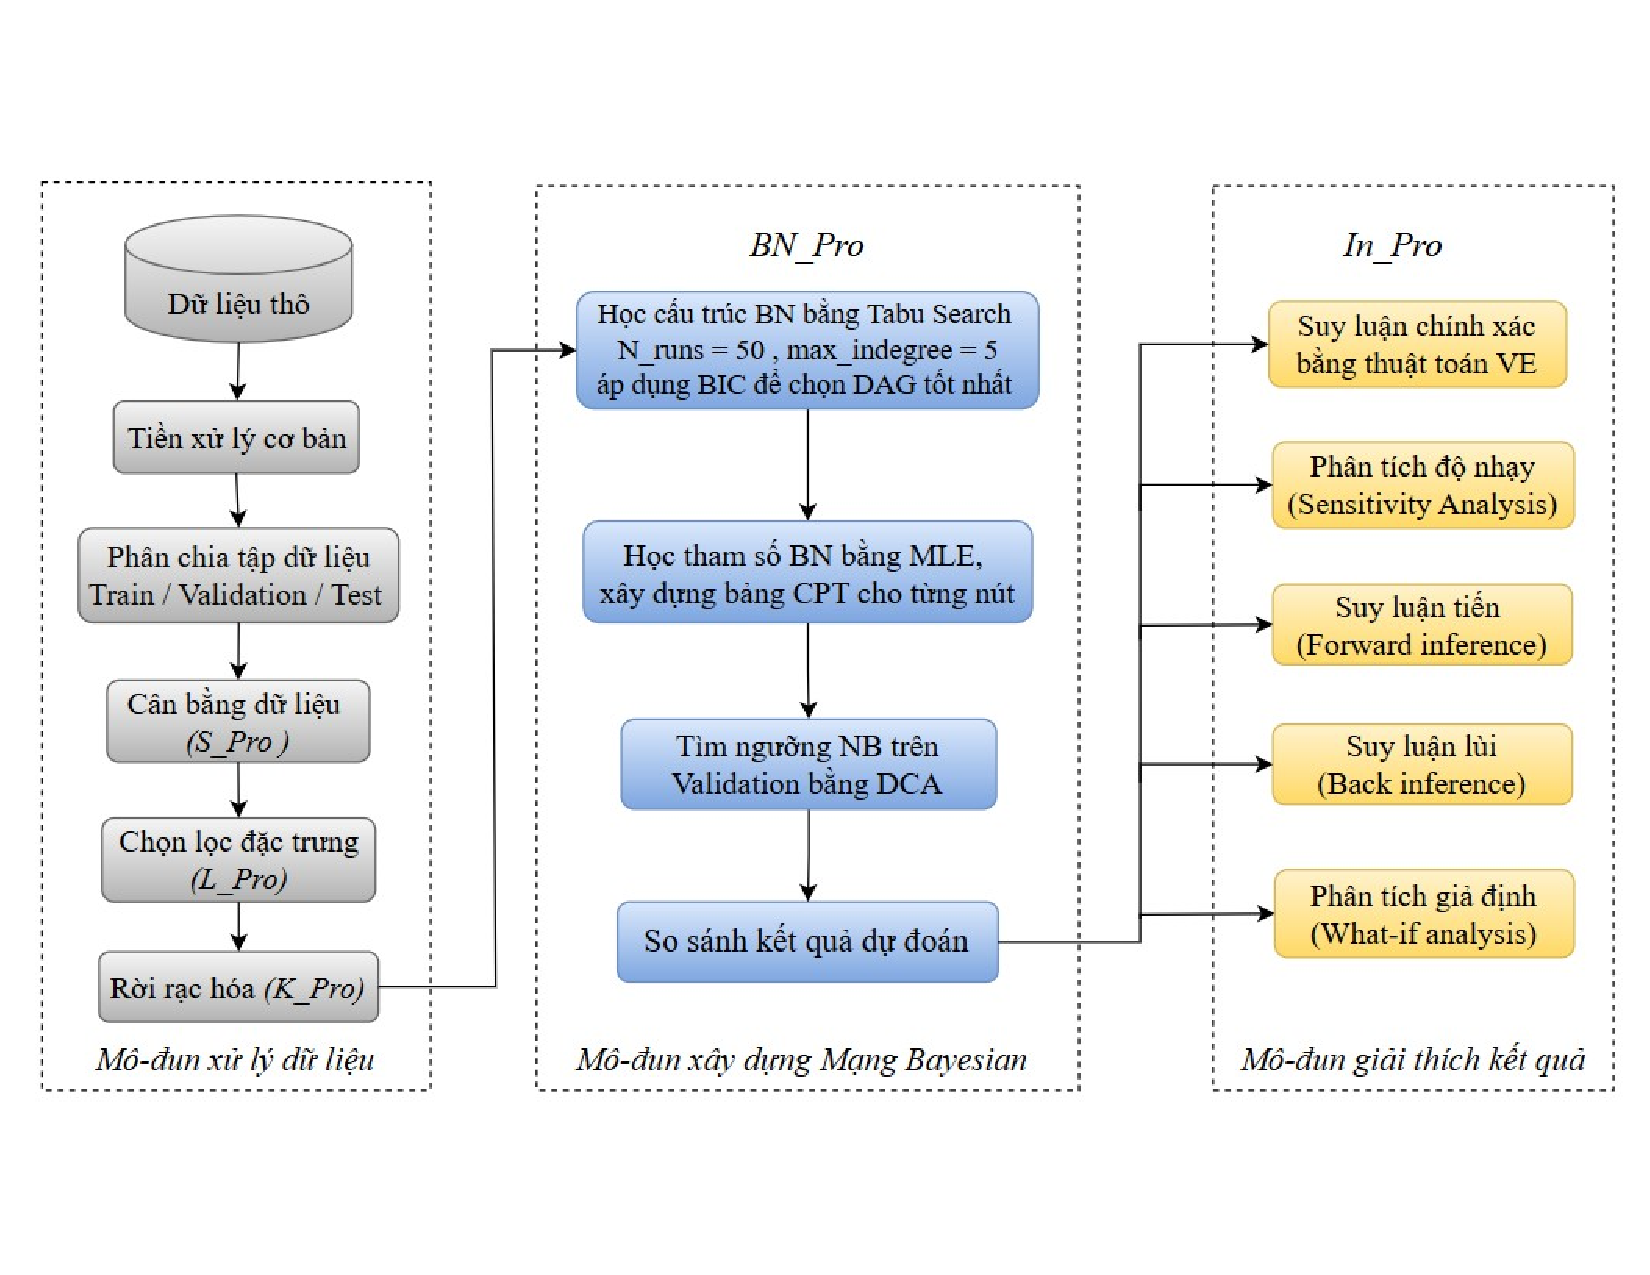
\includegraphics[width=1.05\textwidth,
    trim=0.5cm 2cm 0cm 3cm,
    clip]{image/frame.pdf}
    \caption{Framework of the proposed model.}
    \label{fig:framework}
\end{figure}
\FloatBarrier

\subsection{Data Processing Procedure}
\subsubsection{Data Balancing with SMOTE (S\_Pro)}
\noindent
In the credit risk prediction problem, the training dataset often exhibits severe class imbalance, with the number of default profiles (the minority class) considerably smaller than that of ordinary profiles (the majority class) (Table \ref{tab:dataset_summary}, Figure \ref{fig:class_imbalance}). Without intervention, machine learning algorithms tend to be biased towards the majority class, resulting in a distorted decision boundary and a severe reduction in the ability to identify genuine risk. To remedy this, the present study applies the Synthetic Minority Over-sampling Technique (SMOTE) in order to rebalance the class distribution before the data enters the Bayesian network structure learning procedure.
SMOTE operates by synthesising new minority samples rather than directly duplicating existing observations, thereby avoiding local overfitting \cite{chawla2002smote}. Specifically, for each minority sample $x_i$, the algorithm identifies the $k$ nearest neighbours in the feature space according to Euclidean distance, then randomly interpolates along the line segment joining $x_i$ to a randomly chosen neighbour $x_{nn}$ in order to create a new synthetic sample $x_{\text{new}}$ according to the formula:
\begin{equation}
    \label{eq:3.1}
    x_{\text{new}} = x_i + \lambda \cdot (x_{nn} - x_i), \quad \lambda \sim \mathcal{U}(0, 1)
\end{equation}
where $\lambda$ is a random value sampled uniformly from the interval $[0, 1]$. This process is repeated until the number of samples in the minority class is balanced with that of the majority class. The algorithm is presented as follows:

\vspace{0.5em}
\begin{algorithm}
\caption{Pseudocode of the SMOTE algorithm}
\vspace{0.5em}
\textbf{Input:} Minority sample set $X_{min}$, number of neighbours $k$, synthesis ratio $N$.

\vspace{0.5cm}
\textbf{Output:} Synthetic sample set $X_{syn}$.
\begin{tcolorbox}
\begin{algorithmic}[1]
    \State $X_{syn} \gets \emptyset$
    \For{each $x_i \in X_{min}$}
        \State Compute the $k$ nearest neighbours of $x_i$ in $X_{min}$ according to Euclidean distance
        \For{$n = 1$ to $N$}
            \State Randomly select $x_{nn}$ from the set of $k$ neighbours
            \State Sample $\lambda \sim \mathcal{U}(0, 1)$
            \State $x_{new} \gets x_i + \lambda \cdot (x_{nn} - x_i)$
            \State $X_{syn} \gets X_{syn} \cup \{x_{new}\}$
        \EndFor
    \EndFor
    \State \textbf{return} $X_{syn}$
\end{algorithmic}
\end{tcolorbox}
\end{algorithm}

The key point of the interpolation mechanism is that the synthetic samples created lie on the line segment joining two real samples in the feature space, and therefore always fall within a neighbourhood of genuine data density. This ensures that new samples are not generated in regions of space far removed from the original distribution, a common drawback of synthesis methods based on random noise. As a result, the decision boundary between the two classes is expanded and smoothed more naturally, helping the model to learn the discriminative characteristics of the minority class rather than merely memorising repeated samples.

\subsubsection{Feature Selection Using Lasso Regression (L\_Pro)}
\label{sec: 3.1.2}
\noindent
After the data balancing stage, the input feature space often contains many variables with low contribution or high mutual correlation, causing information redundancy and increasing the computational cost of the Bayesian network structure learning process — which is already an NP-hard problem. The feature selection step therefore plays an important role in reducing the dimensionality of the variable space while still preserving the discriminative power of the model.
This study applies Logistic regression with L1 regularisation (commonly referred to as Lasso regression) as the principal feature selection mechanism. Mathematically, Lasso adds to the objective function a penalty term proportional to the sum of the absolute values of the coefficients, forcing the coefficients of certain variables exactly to $0$ when the improvement in model fit from including a variable is not sufficient to offset its penalty in increasing the number of probability parameters to be estimated, thereby performing automatic feature selection within the parameter estimation process itself \cite{tibshirani1996lasso}. The corresponding optimisation problem is written as:

\vspace{1em}
\begin{equation}
    \hat{\beta} = \arg\min_{\beta} \left[ -\ell(\beta; \mathbf{X}, \mathbf{y}) + \frac{1}{C} \sum_{j=1}^{p} |\beta_j| \right],
\end{equation}
\noindent
where,
\begin{itemize}
    \item $\hat{\beta}$: The optimal set of coefficients (weights) to be estimated for the model.
    \item $\ell(\beta; \mathbf{X}, \mathbf{y})$: The log-likelihood function of the logistic model with respect to the feature matrix $\mathbf{X}$ and the vector of actual labels $\mathbf{y}$. 
    \begin{equation}
        \ell(\beta; \mathbf{X}, \mathbf{y}) = \sum_{i=1}^{n} \Big[ y_i \log p_i + (1 - y_i) \log (1 - p_i) \Big], \qquad p_i = \frac{1}{1 + e^{-\boldsymbol{\beta}^\top \mathbf{x}_i}}
    \end{equation}
    \item $\beta_j$: The weight coefficient corresponding to the $j$-th feature in the data.
    \item $p$: The total number of input features.
    \item $C$: The inverse of the penalty strength ($C > 0$), used to control the degree of regularisation of the model:
    \begin{itemize}
        \item \textit{When $C$ is small:} The strong penalty forces many coefficients $\beta_j$ decisively to $0$; specifically, a variable is eliminated when the improvement it brings to the log-likelihood function is smaller than the penalty that $L_1$ regularisation imposes on its coefficient, that is, when the marginal contribution of the variable is not sufficient to justify its retention in the model.
        \item \textit{When $C$ is large:} The penalty is weak, and the objective function tends towards the form of ordinary logistic regression without constraints.
    \end{itemize}
    \item $\sum_{j=1}^{p} |\beta_j|$: The L1 regularisation term (L1 norm), measuring the sum of the absolute values of the coefficients.
\end{itemize}

\subsubsection{Data Discretisation Using K-means (K\_Pro)}
\label{sec: 3.1.3}
\noindent
Bayesian networks require the input variables to be in discrete form so that conditional probability tables can be constructed through frequency statistics. When the data contains continuous variables, computing conditional probabilities directly over a continuous value domain is computationally infeasible and also leads to severe data sparsity in the cells of the CPT \cite{koller2009probabilistic}\cite{friedman1996discretizing}. The discretisation step is therefore a prerequisite for ensuring the validity of the network parameter learning process.

This study uses the K-means algorithm as its principal discretisation mechanism \cite{liu2024credit}. To understand the reason for this choice, we consider the differences between three common discretisation strategies. The equal-width method divides the entire value domain into $k$ intervals of equal width, regardless of the actual density of the data distribution. As a consequence, the bins in the tail regions of financial data distributions, which are typically strongly skewed, will contain very few observations, leading to unreliable estimates of conditional probability in the CPT. The equal-frequency method overcomes the density problem by ensuring that each bin contains approximately the same number of observations, but it may sever the natural clusters in the data when bin boundaries are placed arbitrarily according to quantiles. K-means, by contrast, divides the value domain on the basis of the actual geometric density structure, seeking bin boundaries such that the observations within the same bin are as similar to one another as possible. This is particularly meaningful for Bayesian networks, since more homogeneous bins produce CPT cells that more accurately reflect the true data-generating mechanism.

With $k$ bins determined in advance, K-means seeks a set of cluster centroids $\{\mu_1, \mu_2, \dots, \mu_k\}$ that minimises the total within-cluster sum of squared distances \cite{macqueen1967methods}:
\begin{equation}
    \label{eq: 3.3}
    \min_{\{S_i\}} \sum_{i=1}^{k} \sum_{x \in S_i} (x - \mu_i)^2,
\end{equation}

\noindent
where:
\begin{itemize}
    \item $k$: The total number of clusters (the number of bins) defined in advance.
    \item $S_i$: The set of data points (observations) assigned to the $i$-th cluster.
    \item $x$: A particular data point with a continuous value belonging to cluster $S_i$.
    \item $\mu_i$: The centroid of the $i$-th cluster, usually the mean value of all points $x$ lying within that cluster.
    \item $(x - \mu_i)^2$: The squared distance from the data point $x$ to its corresponding cluster centroid $\mu_i$.
\end{itemize}

In the centroid update step, the centroid of each cluster is recomputed as the arithmetic mean of all the points belonging to that cluster. This iterative process is guaranteed to converge because the objective function is non-negative and decreases monotonically after each iteration. The assignment step does not increase the total sum of squared distances, and the centroid update step likewise does not increase the value of the objective function, since the arithmetic mean is the minimiser of the sum of squared distances within a cluster. Each observation is then assigned the bin label corresponding to the index of the nearest cluster, converting the continuous value into a discrete ordinal variable $\{0, 1, \dots, k-1\}$ suited to the input requirements of the Bayesian network. The pseudocode of the algorithm is presented as follows:

\vspace{0.5em}
\begin{algorithm}[H]
\caption{Pseudocode of the K-means algorithm for discretisation}
\label{alg:kmeans_discretization}

\vspace{0.5em}
\textbf{Input:} Dataset $X$, number of bins $k$.

\vspace{0.5cm}

\textbf{Output:} Bin label $b(x) \in \{0, 1, \dots, k-1\}$ for each observation.

\begin{tcolorbox}
\begin{algorithmic}[1]
    \State Initialise $k$ cluster centroids $\{\mu_1, \mu_2, \dots, \mu_k\}$ randomly from $X$
    \Repeat
        \State \textbf{Assignment step:} $S_i \gets \{x \in X : |x - \mu_i| \leq |x - \mu_j|, \forall j \neq i\}$
        \State \textbf{Centroid update step:} $\mu_i \gets \frac{1}{|S_i|} \sum_{x \in S_i} x$
    \Until{the cluster centroids no longer change}
    \State Assign the bin label $b(x) \gets \arg\min_i |x - \mu_i|$ for each $x \in X$
    \State \textbf{return} $\{b(x)\}$
\end{algorithmic}
\end{tcolorbox}

\end{algorithm}

\subsection{Building the Bayesian Network (BN\_Pro)}
\noindent
Unlike black-box machine learning models such as Random Forest, XGBoost or Deep Neural Networks, which focus solely on optimising a predictive loss function, the Bayesian network aims to model the structure of probabilistic dependence among variables by establishing a qualitative structure through the concept of a directed acyclic graph, thereby allowing the mechanism by which credit risk is formed to be clearly described and probabilistic inference to be performed across the entire system \cite{pearl2009causality}, \cite{koller2009probabilistic}, \cite{darwiche2009modeling}.
A DAG is defined mathematically as a graph pair $G = (V, E)$, in which $V$ is the set of vertices representing the random variables in the credit model, and $E$ is the set of directed edges expressing the relationships of direct dependence between pairs of variables. The acyclicity property plays a foundational role, ensuring that if one starts from any node and moves along the direction of the arrows, there never exists a closed path in the system returning to the initial node. In the credit risk prediction problem, this property completely eliminates causal loops that are illogical in economic terms, while also establishing a clear structural ordering among the influencing factors, for example from demographic characteristics and financial history to repayment behaviour and finally to the state of default (Liu et al., 2024) \cite{liu2024credit}.
Applying Bayesian networks to credit risk prediction requires an extremely rigorous model construction procedure that transforms raw financial datasets into a system of causal knowledge capable of mathematical inference. According to Liu et al. (2024) \cite{liu2024credit}, the procedure for building the BN\_Pro model for the credit default prediction problem comprises three core stages: structure learning, estimation of the parameter space, and deployment of the probabilistic inference algorithm. These are three architectural layers tightly linked to one another. The structure learning stage aims to discover the dependency relationships among the variables in the data; the parameter learning stage quantifies the degree of that dependence through conditional probabilities; and the inference stage uses all the knowledge that has been learned to compute the probability of the target event occurring, such as the likelihood that a customer defaults (Default = 1). The organic combination of these three stages fundamentally resolves the barrier of computational complexity that always exists in multidimensional data spaces, while maximising the explanatory capacity of the model in the face of complex credit-granting decisions.
The learning process of a Bayesian network is not merely the optimisation of a predictive function as in Logistic Regression or Gradient Boosting, but the construction of a complete probabilistic model for the entire data system. This forms the foundation for interpretability, sensitivity analysis, counterfactual analysis and causal inference in modern financial research \cite{pearl2009causality}, \cite{liu2024credit}, \cite{peters2017elements}.


\subsubsection{Network Structure Learning}
\noindent
The process begins with determining the network structure, which the academic community has established as an NP-hard problem owing to the exponential explosion of the space of Directed Acyclic Graphs as the number of feature variables increases \cite{koller2009probabilistic}, \cite{jensen2007bayesian} . To overcome this computational barrier, instead of using exhaustive search methods over the entire space, which are infeasible in terms of resources, the structure learning process gives priority to heuristic search algorithms for approximating the globally optimal solution. Within the framework of this study, the Tabu Search algorithm proposed by Glover (1986) \cite{koller2009probabilistic} is deployed as a breakthrough local search tool, combined with the Bayesian information criterion in order to shape a causal network that both fits the data closely and remains structurally parsimonious \cite{liu2024credit}.

The essence of the Tabu Search algorithm is that it fundamentally overcomes the fatal weakness of ordinary hill climbing algorithms, namely becoming trapped at local optima. The algorithm operates by continuously traversing neighbouring graphs through spatial transformations such as adding an edge, deleting an edge or reversing the direction of an arrow. The core difference is the mechanism of maintaining a Tabu list that acts as a short-term memory; when a network structure or a transformation operation has just been evaluated, it is placed on this list and forbidden from being repeated for a certain number of iterations \cite{spirtes2000causation}. This enforcement mechanism prevents the algorithm from returning to previous moves, compelling the system to cross the valleys of the descending function in order to escape the local optimum trap and explore new regions of the structure space, thereby approaching the globally optimal structure \cite{liu2024credit}.

To evaluate the quality of each neighbouring structure during the traversal, the BIC score function is integrated as the ultimate objective function \cite{koller2009probabilistic}. The BIC score acts as a balancing mechanism, resolving the strict trade-off between the goodness of fit of the model (measured by the residual sum of squares or the Likelihood function) and the complexity of the model (measured by the number of free parameters) \cite{liu2024credit}. By imposing a logarithmic penalty on the network size and the number of samples, the BIC criterion effectively prevents overfitting and eliminates edges that cause an unnecessary explosion of parameters.

\begin{equation}
    BIC = \log P(D|\hat{\theta},G) - \frac{\log N}{2}\cdot k,
\end{equation}

\noindent
where:

\begin{itemize}
    \item \(D\): the training data.
    \item \(G\): the DAG structure.
    \item \(\hat{\theta}\): the optimal parameter set of the network.
    \item \(\log P(D|\hat{\theta},G)\): the Log-Likelihood, assessing the ability of the DAG to explain the data 
    \item \(N\): the number of samples.
    \item \(k\): the number of parameters to be estimated.
\end{itemize}
with $\frac{\log N}{2}\cdot k$ being the penalty coefficient for model complexity.

\vspace{1em}
This entire discovery process is placed within a meta-loop of 50 independent network initialisations and training runs in order to eliminate the risk of bias due to the initial starting point, ensuring that the final causal structure reflects the mechanism generating credit risk as faithfully and robustly as possible \cite{liu2024credit}. 

\begin{equation}
G^* = \arg\max_{r=1,...,50} BIC_r,
\end{equation}
where:

\begin{itemize}
    \item $G^*$: the optimal DAG structure selected.
    \item $r = 1,...,50$: the index of the models/DAG structures tested.
    \item $BIC_r$: the BIC score of the $r$-th model.
\end{itemize}

\vspace{1em}
\noindent

The construction and adjustment process is described in Algorithm \ref{alg:tabu_bic}.

\vspace{0.5em}
\begin{algorithm}[h]
\caption{Pseudocode of the BIC-based Tabu Search algorithm}
\label{alg:tabu_bic}
\vspace{0.5em}
\textbf{Initialisation:} A discrete Bayesian network in DAG form. 
Generate a random initial DAG as the current solution. 
Set the current best solution = the current solution = the DAG. 
Initialise the Tabu list and the BIC score.

\vspace{0.5cm}

\textbf{Output:} Return the Bayesian network structure with the highest BIC score.

\begin{tcolorbox}
\begin{algorithmic}[1]
\While{(the stopping criterion has not been met)}
    \State Generate feasible neighbouring network structures.
    \For{(each feasible neighbouring solution $N$)}
        \If{$N$ is not on the Tabu list}
            \State Compute the evaluation index $Q(N)$ of the neighbouring solution $N$ using the BIC score.
            \If{$Q(N) > Q$(the current optimal solution)}
                \State Update the current solution $= N$.
            \EndIf
        \EndIf
    \EndFor
    \State Select the neighbouring solution with the largest $Q(N)$ as the new current solution.
    \State Add the current solution to the Tabu list.
    \State Decrease the Tabu memory of the solutions already in the Tabu list by one unit.
\EndWhile

\State Repeat the Tabu Search algorithm several times with different initial DAGs.
\State Return the DAG with the highest BIC score.
\end{algorithmic}
\end{tcolorbox}
\end{algorithm}
\FloatBarrier

\subsubsection{Parameter Estimation}
\noindent
After the structure learning process has been completed and the directed acyclic graph determined, the Bayesian network has so far only represented the relationships of probabilistic dependence among the variables in the form of a graph structure. The DAG by itself, however, is not sufficient for performing probabilistic inference or predicting credit risk. For the Bayesian network to become a complete probabilistic model, as soon as the DAG skeleton has been firmly established, the system enters the parameter learning stage in order to quantify the causal space \cite{darwiche2009modeling}. The central task is to determine the Conditional Probability Tables for each network node, thereby delineating the degree of statistical dependence among the financial variables \cite{jensen2007bayesian}. This process operates on the basis of Maximum Likelihood Estimation (MLE), a canonical mathematical foundation that allows the observed frequencies from the historical dataset to be transformed directly into predictive probability distributions \cite{liu2024credit}.

According to the Bayesian network theory presented by Pearl \cite{pearl2009causality} and by Koller and Friedman \cite{koller2009probabilistic}, each edge in the DAG reflects only the existence of a relationship of probabilistic dependence between two variables, while the strength and quantitative nature of that relationship is encoded through the probability parameters in the CPT. Hence, if structure learning answers the question ``which variable influences which'', parameter learning answers the question ``how great the influence is'' \cite{pearl2009causality}, \cite{koller2009probabilistic}. 

Consider a Bayesian network comprising a set of $n$ random variables: \textbf{\textit{X}} = $(X_1,X_2,\ldots,X_n)$ with a known DAG structure.
According to the probability decomposition rule of Bayesian networks \cite{pearl2009causality}, \cite{koller2009probabilistic}, \cite{darwiche2009modeling}:
\begin{equation}
    P(X_1,X_2,...,X_n) = \prod_{i=1}^{n} P(X_i \mid Pa(X_i)),
\end{equation}


\noindent
where:

\begin{itemize}
    \item $X_i$ is the $i$-th variable in the network;
    \item$Pa(X_i)$ denotes the set of direct parent nodes of $X_i$;
    \item$P(X_i|Pa(X_i))$ is the probability of the variable $X_i$ given the states of its parent variables in the DAG.
\end{itemize}

\vspace{1em}
The expression above shows that the joint probability distribution of the entire system is decomposed into a product of local probability distributions.

In the credit risk prediction problem, this means that a customer's probability of default is not modelled directly by a single global function, but is derived from the combination of many conditional probabilities among the financial variables, credit behaviour, borrowing history and the target variable Default \cite{liu2024credit}, \cite{masmoudi2019credit}, \cite{leong2016credit}.

\vspace{1em}
\noindent
\textbf{Conditional Probability Table}

\noindent
Suppose the variable $X_i$ has $s_i$ different states.
Its parent set $Pa(X_i)$ has $q_i$ value configurations.
The parameter set to be learned is then:
$$\theta= \{ \theta_{ijk} | i = 1,\dots, n; j = 1,\dots, q; k = 1, \dots, s_i \}$$
with:
\begin{equation}
    \theta_{ijk} = P(X_i=k|Pa(X_i)=j),
\end{equation}

\noindent
where:

\begin{itemize}
    \item $i$: the variable under consideration.
    \item$j$: the $j$-th configuration of the parent set.
    \item $k$: the $k$-th state of the variable.
\end{itemize}

\vspace{1em}
According to Jensen and Nielsen \cite{jensen2007bayesian}, each row in the CPT must satisfy the normalisation constraint:
$$\sum_{k=1}^{s_i} \theta_{ijk} = 1$$
for all:
$$j=1,\ldots,q_i$$
This ensures that the total probability of all possible states of a variable always equals 1.

\vspace{1em}
\noindent
\textbf{The Likelihood Function}

\noindent
Analytically, the algorithm seeks the optimal parameter set such that the likelihood function attains its maximum value. In order to handle the enormous computational load, the algorithm converts the likelihood function into logarithmic form (the log-likelihood), turning complex products of simultaneous probabilities into a series of linear additions \cite{koller2009probabilistic}, \cite{liu2024credit}. By scanning the entire dataset, counting the number of samples satisfying the joint condition between the current node and its parent set, and applying the method of Lagrange multipliers to resolve the mathematical constraints, the system fills in the CPT with precisely the optimal probability percentages \cite{liu2024credit}. The resulting parameter grid not only describes the structure of the training data but also becomes the core quantitative knowledge base for every subsequent inference query \cite{darwiche2009modeling}, \cite{liu2024credit}. 

\vspace{1em}
\noindent
Suppose the training dataset:
$$D={d_1,d_2,\ldots,d_m}$$
consists of $m$ independent observations.

\vspace{1em}
According to Koller and Friedman \cite{koller2009probabilistic}, the likelihood function is defined as:
\begin{equation}
    L(\theta|D) = P(D|\theta) = \prod_{l=1}^{m} P(d_l|\theta),
\end{equation}
where:
\begin{itemize}
    \item $L(\theta|D)$: the likelihood function, representing the probability of observing the data $D$ given the parameters $\theta$.
    \item $D$: the training dataset.
    \item $\theta$: the parameter set of the Bayesian network.
    \item $P(d_l|\theta)$: the probability of the $l$-th data sample given the parameter set $\theta$.
    \item $m$: the total number of data samples in the training set.
\end{itemize}

    
\vspace{1em}
\noindent
The objective of MLE is to find the parameter set:
$$\theta^* = \arg\max_{\theta} L(\theta|D)$$
that is, the parameter set that makes the observed data most probable.

\vspace{1em}

Because the likelihood function is a product of a great many small probabilities, it is prone to arithmetic underflow. Studies on Bayesian networks therefore all switch to the log-likelihood \cite{koller2009probabilistic}, \cite{darwiche2009modeling}, \cite{liu2024credit}.

\vspace{1em}
Let $m_{ijk}$ denote the number of samples satisfying: $X_i=k$ and $Pa(X_i)=j$ 

Then:
\begin{equation}
\begin{aligned}
\label{eq: log}
\ell(\theta|D) 
&= \log L(\theta|D) \\
&= \log \prod_{l=1}^{m} P(d_l|\theta) \\
&= \sum_{i=1}^{n} \sum_{j=1}^{q_i} \sum_{k=1}^{s_i}
m_{ijk} \log(\theta_{ijk}),
\end{aligned}
\end{equation}
where:
\begin{itemize}
    \item $\ell(\theta|D)$: the log-likelihood function of the Bayesian network with parameter set $\theta$ and data $D$.
    \item $n$: the number of variables in the Bayesian network.
    \item $q_i$: the number of states of the parent set of the variable $X_i$.
    \item $s_i$: the number of states of the variable $X_i$.
    \item $m_{ijk}$: the number of times the variable $X_i$ is observed in state $k$ while the parent set is in state $j$.
    \item $\theta_{ijk}$: the conditional probability of the variable $X_i$ being in state $k$ given the $j$-th parent state.
\end{itemize}

\vspace{1em}
In order to maximise the log-likelihood function $\ell(\theta|D)$ in formula \ref{eq: log}, the probability normalisation constraint must be satisfied for each node $X_i$ and each combination of parent states $j$:
\begin{equation}
    \sum_{k=1}^{s_i} \theta_{ijk} = 1, \quad \forall i \in \{1,\ldots,n\},\ \forall j \in \{1,\ldots,q_i\}
\end{equation}

\vspace{1em}
This is an optimisation problem with equality constraints, and the method of Lagrange multipliers is therefore applied. The Lagrangian function is constructed as follows:
\begin{equation}
    \mathcal{L}(\theta, \lambda) = \sum_{i=1}^{n}\sum_{j=1}^{q_i}\sum_{k=1}^{s_i} m_{ijk}\log(\theta_{ijk})\ +\ \sum_{i=1}^{n}\sum_{j=1}^{q_i} \lambda_{ij}\!\left(1 - \sum_{k=1}^{s_i}\theta_{ijk}\right)
\end{equation}
where $\lambda_{ij}$ is the Lagrange multiplier corresponding to the constraint at node $X_i$ and the $j$-th combination of parent states.

\vspace{1em}
\noindent
Taking the partial derivative of $\mathcal{L}$ with respect to $\theta_{ijk}$ and setting it equal to 0:

\begin{equation}
    \frac{\partial \mathcal{L}}{\partial \theta_{ijk}} = \frac{m_{ijk}}{\theta_{ijk}} - \lambda_{ij} = 0 \implies \theta_{ijk} = \frac{m_{ijk}}{\lambda_{ij}}
\end{equation}

\vspace{1em}
\noindent
Substituting into the normalisation constraint to determine $\lambda_{ij}$:

\begin{equation}
    \sum_{k=1}^{s_i}\theta_{ijk} = \sum_{k=1}^{s_i}\frac{m_{ijk}}{\lambda_{ij}} = \frac{1}{\lambda_{ij}}\sum_{k=1}^{s_i}m_{ijk} = 1 \implies \lambda_{ij} = \sum_{k=1}^{s_i}m_{ijk} = m_{ij\cdot}
\end{equation}
where $m_ij = \sum_{k=1}^{s_i}m_{ijk}$ is the total number of observations whose parent set is in state $j$, regardless of the state of $X_i$.

\vspace{1em}
\noindent
Substituting back, the explicit solution of the MLE problem is:
\begin{equation}
    \boxed{\hat{\theta}_{ijk} = \frac{m_{ijk}}{m_{ij\cdot}}}
\end{equation}

\vspace{1em}
This solution has a clear intuitive meaning: the optimal conditional probability of $X_i$ being in state $k$ when the parent set is in state $j$ is precisely the relative frequency observed in the training data. This is the mathematical basis on which the MLE class in the pgmpy library fills in the values of the CPT: instead of iterative optimisation, it need only count the frequency of occurrence of each combination of states $(X_i = k, Pa(X_i) = j)$ in the training set and compute the ratio. This is the central formula of the entire parameter learning process in Bayesian networks \cite{koller2009probabilistic}, \cite{liu2024credit}.

\subsubsection{Initialising the Inference Mechanism and Markov Blanket Analysis}
\noindent
Immediately after the complete Bayesian network has been built, an exact inference engine based on the variable elimination algorithm is initialised in conjunction with the model, serving as the sole interface through which all probabilistic queries in the In\_Pro phase will pass. Before exploiting the inference mechanism for prediction and explanation purposes, a preliminary sanity check is carried out: the unconditional prior probability P(target = 1) is queried directly from the Variable Elimination engine and compared against the empirical prior probability prior\_default computed directly from the frequencies in the training data. Agreement between these two values (with a discrepancy smaller than a conventionally agreed tolerance threshold) is a necessary (though not sufficient) condition for asserting that the graph structure and the learned Conditional Probability Distributions (CPD) correctly encode the latent dependency relationships in the original data, since if inference over the network cannot exactly reproduce the marginal distribution of the target variable that was used to learn those parameters, there is a high likelihood of an error in constructing the graph or in estimating the CPT.
In parallel with this validation step, an important structural analysis is performed, namely determining the Markov Blanket set of the target variable, denoted MB(target), which is formally defined as the union of three subsets: the set of direct parents (Parents), the set of direct children (Children), and the set of parents of the children (Parents of Children, also known as the set of ``spouses''):
$$MB(target) = Parents(target) \cup  Children(target) \cup Parents(Children(target))$$
According to Pearl's definition \cite{pearl2009causality} within the framework of Bayesian networks, the core theoretical significance of the Markov Blanket is the property of conditional independence separation: once the states of all the variables in MB(target) are known, the target variable becomes conditionally independent of every remaining variable in the network that does not belong to the Markov Blanket 
\[
\textit{target} \perp (\textit{all other variables}) \mid \textit{MB(target)}
\]
\vspace{1em}
The direct practical consequence of this property is that the Markov Blanket is precisely the minimal and sufficient feature set required to predict the target variable accurately within the framework of the learned model: adding any variable outside MB(target) to the evidence set of an inference query will not contribute any additional marginal information for estimating P(target | evidence), because the entire influence of those variables (if any) has already been transmitted and fully ``absorbed'' through the intermediate variables belonging to the Markov Blanket. This is the theoretical basis for the study's use of the Markov Blanket as a tool for structural explanation, running in parallel with the specific probabilistic inference analyses in the In\_Pro phase.

\subsection{Interpretation of Results (In\_Pro)}
\noindent
Successfully constructing a Bayesian network does not stop at prediction; the graph structure must also be fully exploited in order to explain the mechanism by which risk is formed. The Interpretation Process (In\_Pro) block serves as a bridge between the computational power of machine learning and the human need to understand root causes. This stage operates mainly on two core foundations: the mechanism of multidimensional probabilistic inference and the technique of sensitivity analysis combined with mutual information.

\subsubsection{Exact Inference Using the Variable Elimination Algorithm}
\noindent
Once the Bayesian network has been completed in terms of both its qualitative geometric structure and its quantitative parameter system, the next core problem is to exploit the model in order to produce scientific judgements when real-world information appears. This process is called probabilistic inference, in which the system updates the probability distribution of one or a group of target variables given the specific known states of another group of observed variables, which serve as empirical evidence (Liu et al., 2024) \cite{liu2024credit}. Within the scope of rigorous mathematical methods, exact inference is the approach that computes posterior probability values that are absolute and analytically precise, rather than using stochastic approximation techniques that carry uncertainty. The results of exact inference ensure that every risk decision made rests on a purely mathematical logical foundation, unaffected by simulation error.

In the context of credit risk prediction research, the ultimate goal is not to determine the probability of each individual variable but to infer the probability of a customer defaulting given an observed set of specific credit information. This is equivalent to computing the posterior probability:

\begin{equation}
    P(Default=1 \mid X_1=x_1, X_2=x_2, ..., X_m=x_m)
\end{equation}

\noindent
in which the set of observed variables serves as the evidence, while the variable Default serves as the query variable \cite{liu2024credit}.

\vspace{1em}
According to Pearl (2009) \cite{pearl2009causality}, the inference process in a BN is precisely the process of belief updating when new information appears. Mathematically, this is carried out through Bayes' theorem combined with the probability decomposition structure of the network.This form of decomposition is the foundation that allows a BN to handle complex inference problems by exploiting conditional independence. This is precisely the important advantage that makes BNs suitable for the credit risk assessment problem, in which factors such as income, credit history, financial behaviour and loan status are mutually dependent \cite{pearl2009causality}, \cite{koller2009probabilistic}, \cite{darwiche2009modeling}. 

Although the probabilistic representation becomes more efficient, performing exact inference on a Bayesian network remains a problem of very high computational complexity. Cooper (1990) \cite{cooper1990computational} proved that the problem of exact probabilistic inference on a BN belongs to the NP-hard class. This means that the computational cost may grow exponentially as the number of variables or the density of connections in the network increases. For this reason, the choice of an appropriate inference algorithm plays a decisive role in the practical applicability of Bayesian networks in large-scale credit risk prediction systems. 

In the study by Liu et al. \cite{liu2024credit}, as well as in the model \ proposed in this thesis, the Variable Elimination (VE) algorithm is chosen as the exact inference mechanism for computing a customer's probability of default from the learned Bayesian network structure. 

\vspace{1em}
\noindent
\textbf{The Variable Elimination Algorithm}

\noindent
VE is one of the classic exact inference algorithms for Bayesian networks, developed on the ideas of non-sequential dynamic programming and the technique of decomposing the inference problem into local operations on probabilistic factors \cite{darwiche2009modeling}, \cite{jensen2007bayesian}, \cite{dechter1999bucket}.

The core idea of the algorithm is to avoid computing the entire joint probability distribution of the network directly. Instead, VE takes advantage of the graph structure and the relationships of conditional independence to carry out probability additions and multiplications in an optimal order so as to reduce the number of operations that must be performed \cite{darwiche2009modeling}.

\vspace{1em}
Suppose we need to compute:
$$P(Y|E=e)$$ 
where $Y$ is the query variable and $E$ is the set of evidence variables. By the definition of posterior probability:

\begin{equation}
    P(Y \mid E = e) = \frac{P(Y, E = e)}{P(E = e)} = \frac{\sum_{z} P(Y, E = e, Z = z)}{\sum_{y, z} P(Y = y, E = e, Z = z)},
\end{equation}

\noindent
where:
\begin{itemize}
    \item $P(Y \mid E = e)$: The posterior probability of the target state variable $Y$ (for example, the likelihood of default) after the evidence set $E = e$ has been observed.
    \item $Y$, $y$: The target variable to be queried and its specific state.
    \item $E$, $e$: The set of evidence variables in the Bayesian network and the specific values actually recorded (for example, the customer has a low income or a history of late payment).
    \item $Z$, $z$: The set of intermediate variables belonging neither to the target group $Y$ nor to the evidence group $E$, and their state space.
    \item $\sum_z$: The marginalisation summation over the entire state space of $Z$, in order to eliminate the influence of these intermediate variables from the query result.
    \item $\sum_{y, z}$: The summation over the entire state space of both $Y$ and $Z$ in order to compute the marginal probability $P(E = e)$ in the denominator, which acts as a normalising constant ensuring that the total probability equals $1$.


\item $P(E=e)$ is the probability of the evidence occurring
\item $P(Y,E=e)$ is the joint probability of the query variable and the evidence. 
\end{itemize}

\vspace{1em}
If the summation is performed directly over the entire state space of $Z$ $(O(k^n))$, where $k$ is the average number of states per variable and $n$ is the number of hidden variables, the computational cost will grow exponentially. VE resolves this problem by changing the order of the multiplication and summation operations:

$$\sum_Z \prod_i f_i$$
\noindent
into a sequence of local operations:

$$\sum_{Z_k} \left( f_1 \cdot f_2 \cdots f_m \right)$$
\noindent
such that only one intermediate variable $Z_k$ is removed from the system at a time.

It is precisely this interchange of the order of multiplication and summation that allows VE to reduce inference complexity considerably compared with the brute-force method \cite{darwiche2009modeling}, \cite{dechter1999bucket}, \cite{murphy2012machine}. Algorithm \ref{alg:magia_VE} below is the pseudocode of the VE algorithm.

\vspace{1em}
\begin{algorithm}
    \caption{Pseudocode of the variable elimination inference algorithm}
\vspace{0.5em}
\label{alg:magia_VE}

\textbf{Input:} Bayesian network $BN$.

\vspace{0.2cm}

\textbf{Output:} Return the posterior probability $P(Y|E=e)$.

\vspace{0.2cm}
\begin{tcolorbox}
\begin{algorithmic}[1]
\State Initialise the VE inference engine with $BN$.

\vspace{0.1cm}
\State Set the query variable $Y$ and the evidence $E=e$.

\vspace{0.1cm}
\State Extract the factors $F$ from $BN$.

\vspace{0.1cm}
\While{hidden variables remain}

\vspace{0.1cm}
    \State Select a variable $X$ from the elimination order $\rho$.

\vspace{0.1cm}
    \State Multiply the factors containing $X$.

\vspace{0.1cm}
    \State Eliminate $X$ by summation.

\vspace{0.1cm}
\EndWhile

\vspace{0.1cm}
\State Combine the remaining factors to obtain $h(Y)$.

\vspace{0.1cm}
\State Return $P(Y|E=e) = h(Y) \text{/} \sum_Y h(Y)$.

\end{algorithmic}
\end{tcolorbox}
\end{algorithm}

A Bayesian network represents the joint distribution as a product of local CPDs: $P(X_1,...,X_1)$. From the computational standpoint of the VE algorithm, each of these CPDs is regarded as a factor, that is, a function defined over a subset of variables, mapping each combination of states of those variables to a non-negative probability value. A factor $f(A, B, C)$ need not be a normalised probability distribution; it need only be a table of values capable of taking part in multiplication and aggregation operations.

\begin{enumerate}
    \vspace{1em}
    \item \textbf{Factor multiplication}

    When two factors share one or more variables, for instance $f_1(A, B)$ and $f_1(B, C)$, factor multiplication produces a new factor over the union of the participating variables:
    \begin{equation}
        f(A, B, C) = f_1(A, B) \times f_2(B, C)
    \end{equation}
    where, for each specific combination of states of $(A, B, C)$, the value of the resulting factor equals the product of the corresponding values of the two component factors at the shared state combination of the variable $B$. This operation is the basic computational building block that allows the local joint distribution to be reconstructed gradually from the initial discrete CPDs, without explicitly constructing the entire joint distribution table over all variables.


    \vspace{1em}
    \item \textbf{Variable elimination}

    Instead of computing the summation directly over the entire state space of the hidden variables, the VE algorithm marginalises the hidden variables one at a time, immediately after multiplying the factors related to that variable, according to the distributive law of addition over multiplication:
    
    \begin{equation}
        \sum_{\text{hidden}} \prod_i f_i \Rightarrow \sum_{\{Z_1\}} \left(\sum_{\{Z_2\}} \left( ... \left( f_1 \times f_2 \times ... \times f_m \right) ... \right)\right)
    \end{equation}
    
    \hspace{0.5cm} Specifically, for each variable $X_k$ to be eliminated in the predetermined elimination order $\rho=(X_1,X_2,\ldots,X_k)$, the algorithm groups together all the existing factors that still contain $X_k$, multiplies them into an intermediate factor, then sums out $X_k$ from this intermediate factor to obtain a new factor no longer containing $X_k$, and replaces the old factors with this new factor in the set of factors being processed. The process is repeated until all hidden variables have been eliminated, leaving factors containing only the query variable $Y$, which are multiplied together to obtain $h(Y)$ and finally normalised into a valid posterior distribution:
    \begin{equation} 
        P(Y | E = e) = \frac{h(Y)}{\sum_Y h(Y)}
    \end{equation}

\end{enumerate}

The complexity advantage of VE over brute-force enumeration lies in the fact that the aggregation order is arranged so that each aggregation operation acts only on small local factors rather than on the global joint distribution table. However, the computational complexity of VE depends directly on the treewidth of the graph corresponding to a particular elimination order, and finding the elimination order that minimises treewidth is itself an NP-hard problem. In practice, pgmpy applies heuristics for selecting the elimination order based on the smallest node degree (the min-degree heuristic) in order to approximate an efficient elimination order, and with the credit network structure used in this research, the computational cost of VE remains within feasible limits for the repeated queries required by sensitivity and what-if analysis.

\subsubsection{Probabilistic Inference in Bayesian Networks}
\vspace{1em}
\noindent
\textbf{Forward Inference}

\noindent
The core essence of the interpretive power of Bayesian networks lies in their capacity for probabilistic inference, which operates on the firm foundation of Bayes' theorem. Unlike closed algorithms that establish only a one-directional mapping from input to output, the Bayesian network uses the organic relationship between the joint probability distribution function and the conditional probability distribution functions to carry out multidirectional inference. In terms of graph representation, each node in the network stands for a random variable, while the directed edges connecting the nodes depict directly the relationships of conditional dependence among these variables. Accompanying that geometric structure, each node possesses a conditional probability distribution table, which describes quantitatively the shift in the probability distribution at that node when the values of its dependent variables (the parent variables) change. This decomposition allows the system to represent the joint probability of the entire variable space $X = \{X_1, X_2, \dots, X_n\}$ through a product of local probabilities according to the formula:

\begin{equation}
    P(X_1, \dots, X_n) = \prod_{i=1}^n P(X_i | Pa(X_i))
\end{equation}

On the basis of that architecture, the forward inference mechanism is defined as the process of computing the posterior probability distribution of a target variable given evidence provided by one or more feature variables $P(Y|E=e)$. 

Considered in the experimental context of the credit-granting problem, by learning from the historical dataset of individuals who have previously taken out loans, the model can establish the structure and the intrinsic conditional probability distributions among the feature nodes, for example computing the probability that an individual has a borrowing need and a risk of default under the constraining conditions of their current income level and their past credit rating score \cite{liu2024credit}. As soon as the system receives an entirely new application for a personal credit limit, the forward inference process is immediately activated. The empirical values of that individual's income and credit score are assigned directly into the network as evidence variables. Through the Bayesian inference engine, the system propagates probabilities along the directed edges of the graph, thereby automatically computing and outputting the posterior probability distribution expressing that individual's borrowing need as well as their potential default rate \cite{murphy2012machine}. This process is not a mere approximation of a function but a circulation and updating of belief entirely grounded in the laws of statistical probability.

\vspace{1em}
\noindent
\textbf{Backward Inference}

\noindent
In parallel with forward inference, the Bayesian network also provides a superior mathematical basis for backward inference, otherwise known as diagnostic reasoning. In this direction of inference, the algorithm computes the posterior probability distribution of one or more feature variables (causes) once the specific state of one or more target variables (effects) has been observed \cite{pearl2009causality}. For instance, when the system records a profile that has genuinely fallen into the state of default, backward inference will diagnose and reconstruct the probability of occurrence of the income levels or credit behaviours that led to that outcome. 

\vspace{1em}
\noindent
Suppose:
\begin{itemize}
    \item $Y$: the target variable, which in this study is Default.
    \item $X$: the feature variable to be inferred (for example, Income, CreditScore, etc.).
\end{itemize}

\vspace{1em}
Given that the customer has defaulted ($Y=1$), the posterior probability of the feature variable is determined by:
\begin{equation}
    P(X|Y=1) = \frac{P(Y=1|X)\,P(X)} {P(Y=1)},
\end{equation}

\noindent
where:
\begin{itemize}
    \item $P(X|Y=1)$: the posterior probability of the variable $X$ given that the customer has defaulted.
    \item $P(Y=1|X)$: the probability that the customer defaults given the value of $X$.
    \item $P(X)$: the prior probability of the variable $X$.
    \item $P(Y=1)$): the prior probability of the target variable, acting as a normalising constant.
\end{itemize}

\vspace{1em}
The ability to combine forward inference (to predict the future) and backward inference (to diagnose causes) seamlessly is precisely the theoretical reason why Bayesian networks have become the gold standard in artificial intelligence systems specialising in probabilistic inference and financial decision-making \cite{darwiche2009modeling}, \cite{liu2024credit}. By continuously adding and updating new evidence in the observation space, the graph continuously refines the probability distribution curves, thereby sharpening the precision and accuracy of credit judgements in subsequent cycles.


\subsubsection{Sensitivity Analysis Method}
\label{sec: 3.3.3}
\noindent
In order to measure quantitatively and to isolate the mechanism of influence within the network structure, sensitivity analysis is deployed as a key posterior evaluation tool. Within the Bayesian network ecosystem, sensitivity analysis is usually decomposed into two specialised lines of reasoning: structural sensitivity analysis and parameter sensitivity analysis \cite{kamal2021sensitivity}, \cite{rohmer2020sensitivity}. On the structural analysis side, the degree of influence on the target variables is assessed by directly adjusting the network architecture: researchers actively intervene in the geometric skeleton of the DAG through operations such as grafting on, or eliminating, nodes and links (edges). After each structural transformation, the algorithm recomputes the posterior probability distribution and compares it with the original network in order to measure the discrepancy; the larger the discrepancy, the more it demonstrates the acute sensitivity of the target to that structural change. Parameter sensitivity analysis, by contrast, focuses on preserving the graph architecture while actively intervening in the intrinsic parameters of the network, specifically the values inside the conditional probability distribution table.

Within the scope of this study, the focus of the analysis is placed entirely on parameter sensitivity analysis, in order to exploit to the fullest the local interpretability of the model with respect to credit scenarios. By applying the control variable method thoroughly, the researcher can actively change the value of a single input variable (for example, the borrower's income level) while freezing all the remaining variables. By repeating this trial many times and recording the continuous change in the probability of default, the model quantifies precisely the magnitude of that feature's influence on overall risk. The variable that produces the largest shift in probability is precisely the variable with the highest sensitivity. 

\vspace{1em}
Suppose the input variable $X$ changes from the value $x_1$ to $x_2$; the degree of change in the posterior probability is determined by:

\begin{equation}
    \Delta P=P(Y=1|X=x_2)-P(Y=1|X=x_1),
\end{equation}

\noindent
where:
\begin{itemize}
    \item $\Delta P$ is the change in the probability of default;
    \item $X$ is the variable being analysed;
    \item $x_1,x_2$ are two states of the variable.

\end{itemize}

\noindent
The larger $|\Delta P|$ is, the more sensitive that variable is for the predictive model.

\vspace{1em}
Successfully locating the nodes of maximum sensitivity not only provides management with a solid basis for operating the system safely and stably, but also guides purposeful risk intervention measures. At the same time, the results of this process can be used to optimise the model directly by readjusting the weights of the variables or by deciding to collect additional new variables with higher explanatory potential \cite{lin2020behavioral}, \cite{bishop2006pattern} .

To provide a powerful quantitative mathematical basis for determining sensitivity and the degree of association, the study applies the theory of mutual information. In a Bayesian network, mutual information quantitatively expresses the degree of correlation and information sharing between two random variables. Measuring the mutual information between network nodes helps to indicate whether the conditional probability distributions between them are mutually constrained \cite{murphy2012machine}, \cite{cover2006elements}. 

The mathematical formula expressing the mutual information between the feature variable $X$ and the target variable $Y$ is defined as the integral (or the sum, for discrete variables) of the joint distribution function multiplied by the logarithm of the ratio between the joint distribution and the product of the marginal distributions:

\begin{equation}
    I(X;Y) = \sum_{x \in X} \sum_{y \in Y} P(x,y) \log \left( \frac{P(x,y)}{P(x)P(y)} \right)
\end{equation}

\vspace{1em}
If the mutual information between two nodes equals $I(X;Y) = 0$, this is absolute mathematical proof that the two nodes are entirely conditionally independent in the context of the neighbouring nodes already determined. By analysing the mutual information spectrum of the target node, analysts can distil and rank precisely the degree of association between the input feature nodes and the danger of default, thereby eliminating noisy features and establishing an optimal inference space that is extremely convincing for the predictive results.


\subsection{Evaluation of Predictive Performance}

\subsubsection{Receiver Operating Characteristic Curve}
\noindent
In the binary classification problem, the Receiver Operating Characteristic curve (ROC), or ROC curve, is a graphical representation illustrating the performance of a binary classification system as its discrimination threshold is varied continuously over the entire range of possible values. The ROC curve is created by plotting the ratio of true positives to the total number of actual positive samples (TPR) against the ratio of false positives to the total number of actual negative samples (FPR) at different threshold settings [60]. In the context of credit risk prediction, positive is usually taken by convention to be the case of a customer defaulting, while negative is the case of a customer repaying on time (non-default).

The classification model takes as input the customer's financial features and produces a risk score $s$, expressing the degree to which a default event is likely to occur. Based on a classification threshold $c \in (0,1)$, customers are classified into two groups:
\begin{equation}
    \hat{Y}= \begin{cases} 1, & \text{if } s\geq c\\ 0, & \text{if } s<c \end{cases},
\end{equation}
where:
\begin{itemize}
    \item $\hat{Y}=1$: the customer is predicted by the model to be at risk of default (Default).
    \item $\hat{Y}=0$: the customer is predicted by the model not to default (Non-default).
    \item $c$: the classification threshold chosen to convert the continuous risk score into a binary classification decision.

\end{itemize}

\vspace{1em}
After comparing the model's predictions with the customers' actual states, we obtain a Confusion Matrix comprising four cases:

\begin{itemize}
    \item $TP$ (True Positive): the number of customers who actually default and are correctly predicted by the model as defaulting.
    \item $TN$ (True Negative): the number of customers who do not actually default and are correctly predicted by the model as non-defaulting.
    \item $FP$ (False Positive): the number of customers who do not actually default but are incorrectly predicted by the model as defaulting.
    \item $FN$ (False Negative): the number of customers who actually default but are incorrectly predicted by the model as non-defaulting.
\end{itemize}

\vspace{1em}
From the quantities above, the two important components constituting the ROC curve are determined to be sensitivity and the false positive rate (FPR).

\vspace{1em}
Sensitivity, or the rate of correctly detecting defaulting customers, is denoted $Se(c)$ or $TPR(c)$:

\begin{equation}
    TPR(c)=Se(c)=\frac{TP(c)}{TP(c)+FN(c)}
\end{equation}

This quantity reflects the model's ability to identify customers with high credit risk accurately. The larger the value of $TPR(c)$, the fewer potentially defaulting customers the model overlooks.

\vspace{1em}
Conversely, specificity expresses the ability to identify the group of non-defaulting customers accurately:

\begin{equation}
    Sp(c)=\frac{TN(c)}{TN(c)+FP(c)}
\end{equation}

From specificity, the rate at which good customers are wrongly predicted to be risky customers is determined by:

\begin{equation}
    FPR(c)=1-Sp(c)
\end{equation}

or:
\begin{equation}
    FPR(c)=\frac{FP(c)}{FP(c)+TN(c)},
\end{equation}
where:
\begin{itemize}
    \item $FPR(c)$ expresses the proportion of customers who do not default but are misclassified by the model as defaulting at the threshold $c$.
    \item $Sp(c)$ reflects the model's ability to correctly rule out non-risky cases.
\end{itemize}

\vspace{1.5em}

Suppose the risk score output by the model has the corresponding probability density functions:

$$f(s|Y=1) \quad \text{and} \quad f(s|Y=0),$$
where:
\begin{itemize}
    \item $f(s|Y=1)$: the probability density function of the risk score for the group of customers who actually default.
    \item $f(s|Y=0)$: the probability density function of the risk score for the group of customers who do not actually default.
    \item $s$: the risk score predicted by the model.
    
\end{itemize}


\vspace{1.5em}
With a classification threshold $c$, a customer is predicted to default if: $s\geq c$. The probability that the model correctly detects a defaulting customer is then expressed as:
\begin{equation}
    TPR(c)=Se(c)=P(s\geq c|Y=1)
\end{equation}

or:

\begin{equation}
    TPR(c)=\int_{c}^{\infty}f(s|Y=1)ds
\end{equation}

\vspace{1em}
\noindent
Similarly, the probability that the model misclassifies a non-defaulting customer as a defaulting one is determined as:

\begin{equation}
    FPR(c)=P(s\geq c|Y=0)
\end{equation}
or:

\begin{equation}
    FPR(c)=\int_{c}^{\infty}f(s|Y=0)ds
\end{equation}

\noindent
Thus, for each different threshold value $c$, the model produces a pair of values:

$$(FPR(c),TPR(c))$$

\vspace{1em}
When $c$ is allowed to vary continuously over the entire range of the score $s$, the set of these points forms a curve in the two-dimensional space $[0,1]\times[0,1]$. The resulting curve is precisely the ROC curve.

\vspace{1em}
Unlike overall accuracy, the ROC curve does not depend on the prevalence of the default class in the dataset — a key property, since real-world credit data is usually severely imbalanced \cite{chawla2002smote}, with defaulting customers typically accounting for only a small fraction of the whole. At the same time, the ROC curve allows researchers to evaluate classification performance across the entire range of decision thresholds, thereby helping credit institutions to adjust their credit-granting threshold flexibly according to their specific risk appetite, for instance prioritising the minimisation of missed defaulting customers (increasing $Se$) or prioritising the minimisation of wrongful rejection of good customers (increasing $Sp$).


\subsubsection{Area Under the ROC Curve}
\noindent
While the ROC curve provides a comprehensive visual representation of classification performance across all thresholds, it does not directly yield a single aggregate figure for quantitative comparison between models. To address this limitation, the Area Under the ROC Curve (AUC) is introduced as a single scalar measure reflecting the entire discriminative capacity of a classifier across all possible thresholds. The area under a receiver operating characteristic curve, abbreviated AUC, is a single scalar numerical value measuring the overall performance of a binary classifier \cite{hanley1982meaning}.

The landmark theoretical contribution to the statistical interpretation of AUC belongs to Hanley and McNeil (1982) \cite{hanley1982meaning}, who proved an important result: AUC is equivalent in value to the Mann--Whitney U test (also known as the Wilcoxon rank-sum statistic). Given a set of positive samples P and negative samples N, AUC equals the proportion of all (positive, negative) pairs in which the classifier assigns a higher score to the positive sample. This interpretation gives AUC a highly intuitive probabilistic meaning of great practical value: AUC is precisely the probability that the test result of a subject chosen at random from the diseased group (or the defaulting group) exceeds that of a subject chosen at random from the non-diseased group (or the non-defaulting group) \cite{bamber1975area}. Applied to the credit risk problem, this means that AUC reflects the probability that the model assigns a higher risk score to a randomly chosen defaulting customer than to a randomly chosen non-defaulting customer, making it a criterion for evaluating the ranking ability of the model independently of the choice of any particular threshold.

\vspace{1em}
AUC is defined as the integral of the $TPR$ function with respect to $FPR$ over the entire domain $[0,1]$:

\begin{equation}
    AUC = \int_{0}^{1} TPR\big(FPR^{-1}(x)\big) dx = P(S_1 > S_0),
\end{equation}
where:
\begin{itemize}
    \item $S_1$: the risk score assigned by the model to a customer chosen at random from the defaulting group;
    \item $S_0$: the risk score assigned by the model to a customer chosen at random from the non-defaulting group, independent of $S_1$;
    \item $P(S_1 > S_0)$: the probability that a defaulting customer receives a higher score than a non-defaulting customer.
\end{itemize}


\vspace{1em}
In practice, with finite data, AUC is usually estimated through the formula equivalent to the Mann--Whitney U statistic that Hanley and McNeil showed to be:

\begin{equation}
    \widehat{AUC} = \frac{U_1}{n_1 \cdot n_0} = \frac{1}{n_1 n_0}\sum_{i=1}^{n_1}\sum_{j=1}^{n_0} \psi(s_i, s_j)
\end{equation}
with:
\begin{equation}
    \psi(s_i, s_j) = \begin{cases} 1, & \text{if } s_i > s_j \\ 0{.}5, & \text{if } s_i = s_j \\ 0, & \text{if } s_i < s_j, \end{cases}
\end{equation}

\noindent
where:
\begin{itemize}
    \item $n_1$: the number of defaulting customers (positive samples) in the test dataset;
    \item $n_0$: the number of non-defaulting customers (negative samples) in the test dataset;
    \item $s_i$: the risk score of the $i$-th defaulting customer $(i = 1, \dots, n_1)$;
    \item $s_j$: the risk score of the $j$-th non-defaulting customer $(j = 1, \dots, n_0)$;
    \item $U_1$: the Mann--Whitney U statistic computed over the positive--negative sample pairs;
    \item $\psi(s_i, s_j)$: the indicator function comparing each pair of scores, taking the value 1 if the pair is correctly ordered (a concordant pair), 0.5 in the case of a tie, and 0 if incorrectly ordered (a discordant pair).
\end{itemize}

\vspace{1em}
When the data is represented as discrete points on the empirical ROC curve $(FPR_k, TPR_k)_{k=0}^{m}$, AUC can also be computed approximately by the trapezoidal rule:

\begin{equation}
    \widehat{AUC} = \sum_{k=1}^{m} \frac{(TPR_k + TPR_{k-1})}{2} \times (FPR_k - FPR_{k-1})
\end{equation}

\vspace{1em}
Here $m$ is the number of discrete threshold points used to construct the empirical ROC curve. The AUC value lies within the interval [$0.5,1.0$], where the minimum value represents the performance of a random classifier and the maximum value corresponds to a perfect classifier \cite{hanley1982meaning}. Regarding estimation accuracy, Hanley and McNeil (1982) also proposed a closed-form analytical formula for computing the variance of AUC based on the AUC value, the number of positive samples and the number of negative samples, although bootstrap resampling is usually preferred in modern experimental work because it provides better coverage for extreme AUC values \cite{hanley1982meaning}.

In research, AUC serves as the most common benchmark criterion for comparing performance between different models, from classical statistical models such as linear discriminant analysis \cite{altman1968financial} and logistic regression \cite{ohlson1980financial} to modern machine learning models such as random forests \cite{breiman2001random}, support vector machines \cite{vapnik1998statistical}, \cite{shen2022credit} and ensemble methods \cite{breiman1996bagging}, \cite{friedman2001greedy}. Because AUC is independent of the choice of any particular threshold, it allows an objective assessment of the model's intrinsic discriminative capacity before the researcher must make a decision about the optimal classification threshold for practical deployment.

\subsubsection{Criteria for Finding the Optimal Classification Threshold}
\noindent
Although AUC provides a comprehensive measure of the model's discriminative capacity across the entire range of thresholds, in operational practice credit institutions are obliged to select a specific decision threshold $c$ in order to classify customers as granted credit or rejected/placed under risk monitoring. The choice of this threshold cannot be arbitrary but must rest on optimisation criteria with a clear theoretical basis, constructed directly from the geometry and statistics of the ROC curve; in this section we present the mathematical definitions of the methods for determining the optimal threshold that are most commonly used in research on diagnostic accuracy \cite{unal2017defining}. Below is a detailed analysis of the three criteria used in this study.

\begin{enumerate}[label=\alph*)]
    \vspace{1em}
    \item \textbf{The Youden Index Maximisation Criterion}

    The Youden index (Youden's J statistic, or Youden's index) was first introduced by the statistician William J. Youden \cite{youden1950index} in 1950, within the framework of studies aimed at improving the accuracy of medical diagnostic tests. Youden's $J$ statistic is a single number summarising the performance of a binary diagnostic test. It combines sensitivity and specificity into a single index, making it easy to compare tests and to find the optimal decision threshold on a continuous score. Geometrically, the Youden index is precisely the greatest vertical distance between the ROC curve and the reference diagonal (the chance line), that is, the greatest vertical distance between the ROC curve and the chance diagonal, and it is at the same time mathematically equivalent to the Kolmogorov--Smirnov distance statistic\footnote{The Kolmogorov--Smirnov distance statistic is the value measuring the greatest distance between two cumulative distribution functions} measuring the degree of separation between the two score distributions of the defaulting and non-defaulting groups \cite{schisterman2005optimal}.

    \hspace{0.5cm} An important theoretical advantage of the Youden index, which has led to its wide application in credit rating research, is its independence from the prevalence of the positive class in the population. Because it does not depend on the prevalence of the disease, Youden's $J$ index can be transferred between populations with different base rates, unlike predictive values \cite{youden1950index}. This property is particularly well suited to the credit risk prediction problem, where the actual default rate often varies considerably across customer segments, credit products, or stages of the economic cycle.

    \vspace{1em}
    \hspace{0.5cm} The Youden index at the threshold $c$ is defined as:
    \begin{equation}
        J(c) = Se(c) + Sp(c) - 1
    \end{equation}
    and the optimal threshold according to this criterion is determined by:
    \begin{equation}
        c_J = \underset{c \in \mathbb{R}}{\arg\max} J(c),
    \end{equation}
    where:
    \begin{itemize}
        \item $J(c)$: the Youden index at the classification threshold $c$;
        \item $Se(c)$: the sensitivity at the threshold $c$, that is, the proportion of defaulting customers correctly identified by the model;
        \item $Sp(c)$: the specificity at the threshold $c$, that is, the proportion of non-defaulting customers correctly identified by the model;
        \item $c_J$: the optimal classification threshold according to the Youden index maximisation criterion;
        \item $\arg\max_{c}$: the operator finding the value of $c$ that makes the function $J(c)$ attain its maximum over the entire real domain of the threshold.
    \end{itemize}
        \vspace{1em}
        \hspace{0.5cm} The index $J(c)$ takes values in the interval $[-1, 1]$, where $J = 0$ corresponds to a model with no discriminative ability whatsoever (the threshold lies on the reference diagonal of the ROC), while $J = 1$ corresponds to a perfect classification model with neither false positives nor false negatives A $J$ value of zero means that the test provides no useful information, while a value of one indicates perfect classification with no false positives or false negatives \cite{youden1950index}. Youden's $J$ index is one of the oldest and most widely used optimal-threshold frameworks, determining the threshold by maximising the sum of sensitivity and specificity across the different threshold points \cite{unal2017defining}.
        
        \hspace{0.5cm} However, an important theoretical limitation of the Youden criterion was pointed out by Smits (2010) \cite{smits2010note}: maximising $J(c)$ implicitly assumes a misclassification cost ratio equal to $1$ minus the prevalence of the positive class, an assumption that does not always accurately reflect the decision-maker's real priorities.

    
    \vspace{1em}
    \item \textbf{The Closest-to-(0,1) Criterion}

    Also known as the Euclidean distance criterion, formally introduced by Perkins and Schisterman in 2006  \cite{perkins2006inconsistency}, it is based on the geometric intuition that the most ideal operating point on the ROC curve is the point corresponding to a perfect classifier, that is, the point with coordinates $(FPR, TPR) = (0,1)$. Perkins and Schisterman introduced the closest-to-$(0,1)$ criterion, which selects the optimal threshold by minimising the distance of the points on the ROC curve to the perfect classification point $(0,1)$, where both sensitivity and specificity attain their maximum values. In essence this is a direct geometric rule: the optimal threshold is determined at the empirical operating point on the ROC curve with the shortest Euclidean distance to the ideal point $(0,1)$ \cite{ghosal2025impact}.

    \vspace{1em}
    \hspace{0.5cm} The Euclidean distance from the operating point at the threshold $c$ to the ideal point $(0,1)$ is computed as:
    \begin{equation}
        D(c) = \sqrt{\big(1 - Se(c)\big)^2 + \big(1 - Sp(c)\big)^2}
    \end{equation}
    and the optimal threshold according to this criterion is determined by:
    \begin{equation}
        c_{D} = \underset{c \in \mathbb{R}}{\arg\min} D(c)
    \end{equation}
    
    \hspace{0.5cm} This criterion is equivalent to simultaneously minimising the sum of the squares of $FNR (1-Se)$ and $FPR (1 - Sp)$; an estimator based on the smallest sum of squares of 1 minus sensitivity and 1 minus specificity is preferred when sensitivity and specificity are regarded as equally important. Compared with the Youden criterion, the closest-to-(0,1) criterion tends to react more sensitively to asymmetric deviations between the two types of classification error, since it applies a quadratic penalty to the deviation along each axis separately, instead of considering only a linear sum as the Youden index does.
    
    \vspace{1em}
    \item \textbf{The Symmetry Point Criterion}

    The Symmetry Point criterion (the Equal Sensitivity-Specificity Criterion, or the intersection point of the sensitivity and specificity curves) is based on the principle of determining the optimal classification threshold at the position where sensitivity and specificity attain balanced values. When the ROC curve has an area under the curve smaller than one, a trade-off always exists between the ability to correctly detect positive subjects (sensitivity) and the ability to correctly rule out negative subjects (specificity). The optimal threshold can therefore be determined by finding the value of $c$ such that the discrepancy between sensitivity and specificity is smallest.

    \hspace{0.5cm} This approach has a theoretical basis closely related to research on threshold selection when sensitivity and specificity are valued equally, a topic systematically examined in the study by Froud and Abel (2014) \cite{froud2014using} comparing methods for determining the minimally important change threshold in clinical outcome measurement Using ROC curves to select the threshold of minimally important change when sensitivity and specificity are valued equally. The core principle of this group of methods is that, when there is no basis for assigning different cost weights to the two types of classification error ($FP$ and $FN$), the balance point where the two indices $Se$ and $Sp$ are equal is regarded as the fairest and most neutral operating point.

    \vspace{1em}
    \hspace{0.5cm} The optimal symmetry threshold is determined as the solution $c$ of the equation:
    $$Se(c) = Sp(c)$$
    or equivalently, is determined by minimising the absolute deviation between these two quantities:
    \begin{equation}
        c_{S} = \underset{c \in \mathbb{R}}{\arg\min} \big|Se(c) - Sp(c)\big|
    \end{equation}


    \hspace{0.5cm} The threshold $c_{S}$ corresponds to the intersection between the empirical ROC curve and the auxiliary line $TPR+FPR=1$ in ROC space. This criterion has an important practical advantage in the prediction problem. It produces a balanced operating point at which the error rates between the two customer groups (those wrongly rejected and those wrongly granted credit) are equivalent as a percentage within each group, thereby helping credit institutions to maintain a consistent and transparent credit-granting policy that is not excessively biased towards either of the two types of risk (credit risk and the risk of losing customers/business opportunities). It should be noted, however, that the symmetry point criterion, like the Youden criterion, still implicitly assumes cost parity between the two types of classification error, and therefore needs to be applied with consideration for the specific risk management strategy of each financial institution, particularly given that credit data usually exhibits a high degree of class imbalance \cite{chawla2002smote}.


\end{enumerate}

\subsubsection{The Decision Curve Analysis Method}
\noindent
Decision Curve Analysis (DCA) was first formally introduced by Vickers and Elkin \cite{vickers2006decision} in 2006 in the journal \textit{Medical Decision Making}, with the aim of addressing an important gap remaining in traditional methods of evaluating predictive models. While accuracy measures such as sensitivity, specificity and the area under the receiver operating characteristic curve are essential for evaluating predictive models, they cannot capture the practical consequences of deploying such models in the real world. Specifically, measures such as AUC or the Youden index, although they reflect the intrinsic discriminative capacity of the model across the entire range of thresholds, entirely fail to quantify the practical value of a specific decision (for instance the decision to grant or refuse a loan) to the decision-maker, since they treat all classification thresholds as equally important, whereas in reality the consequences of a false positive and a false negative usually carry very different meanings and costs.

The theoretical foundation of DCA stems from formalising the relationship between the decision probability threshold $c$ and the exchange rate between the benefit of a $TP$ and the harm of a $FP$. In the context of credit risk prediction, the concept of the threshold $c$ has a practical interpretation as the minimum probability of default at which a credit institution decides to refuse credit (or to require additional risk mitigation measures such as raising the interest rate or requiring collateral). A low threshold $c$ reflects a prudent credit policy, in which the institution regards the harm of wrongly granting credit to a customer who will default (a false negative in the original logic, or correspondingly ``approve a bad loan'') as far more serious than the harm of wrongly rejecting a good customer; conversely, a high threshold $c$ reflects a credit expansion policy that prioritises maximising the number of loans disbursed and accepts a higher risk of default.

\vspace{1em}
The original formula for Net Benefit proposed by Vickers and Elkin (2006) \cite{vickers2006decision}, computed on a test dataset of $N$ observations, is expressed as follows; in the original paper, the net benefit is computed as:

\begin{equation}
    NB(c) = \frac{TP(c)}{N} - \frac{FP(c)}{N}\left(\frac{c}{1-c}\right),
\end{equation}
where:
\begin{itemize}
    \item $NB(c)$: the net benefit of the model at the decision probability threshold $c$;
    \item $TP(c)$: the number of customers who genuinely default and are correctly predicted by the model at the decision threshold $c$;
    \item $FP(c)$: the number of customers who genuinely do not default but are wrongly predicted by the model as going to default at the decision threshold $c$;
    \item $N$: the total number of observations (customers) in the test dataset;
    \item $\frac{c}{1-c}$: the odds ratio at the threshold $c$, acting as a weighting factor that converts the number of false positives into the same unit of harm as the number of true positives.
\end{itemize}

\vspace{1em}
The formula above is often expressed in an equivalent form in terms of sensitivity, specificity and prevalence, which is more convenient for linking it to the ROC framework presented in the previous sections \cite{vickers2019guide}:

\begin{equation}
    NB(c) = Se(c) \times \pi - \big(1 - Sp(c)\big) \times (1-\pi) \times \frac{c}{1-c}
\end{equation}

The formula above shows that DCA is not a method entirely separate from the ROC framework; rather, it uses the very structural components of the ROC curve ($Se$, $Sp$) as its input material, while adding two elements that ROC/AUC entirely ignore: the actual prevalence of the event ($\pi$) and the relative cost weighting between the two types of error (through the factor $c/(1-c)$) — moving beyond AUC: decision curve analysis to quantify the net benefit of risk prediction models \cite{sadatsafavi2021moving}.

\vspace{1em}
\noindent
\textbf{The Decision Curve and the Reference Lines}

\noindent
After computing $NB(c)$ at a range of different values of $c$ (usually spread evenly over a practically meaningful probability interval, for example from 0.01 to 0.5), plotting $NB(c)$ against $c$ forms the decision curve; plotting the net benefit against the threshold probability produces the decision curve \cite{vickers2006decision}. For the decision curve to have practical interpretive meaning, it is always presented together with two reference strategies serving as comparison standards:

\vspace{1em}
\begin{enumerate}
    \item \textit{Treat All}: assumes that every observation is classified as positive (in the credit context, equivalent to rejecting/monitoring every customer), regardless of the model score. The net benefit of this strategy is computed as:

    \begin{equation}
        NB_{\text{All}}(c) = \pi - (1-\pi)\times\frac{c}{1-c}
    \end{equation}

    \item \textit{Treat None}: assumes that every observation is classified as negative (no customer is rejected on the basis of the model), in which case $TP(c)=FP(c)=0$ and the net benefit is therefore always zero at every threshold; the treat-none strategy assumes that no observation receives the intervention, and by definition its net benefit is always zero across all thresholds:
    
    \begin{equation}
        NB_{\text{None}}(c) = 0 \quad \forall c \in (0,1),
    \end{equation}
    
    \vspace{1em}
    where:
    \begin{itemize}
        \item $NB_{\text{All}}(c) $: the net benefit of the treat-all strategy at the threshold $c$;
        \item $NB_{\text{None}}(c)$: the net benefit of the treat-none strategy at the threshold $c$ (always equal to 0);
        \item $\pi$: the prevalence of the positive class.
    \end{itemize}

\end{enumerate}

A predictive model is considered to have practical value at a specific threshold $c$ if and only if its decision curve lies above both of these reference lines at that threshold; the model provides genuine benefit only within the range of thresholds where its curve lies above both reference strategies. The intersection point of these two reference lines, which occurs precisely at $c = \pi$, carries important guiding significance for determining the range of practically meaningful thresholds to examine in a given study.

Although DCA was developed and popularised mainly in the field of medical statistics, where it has become a routinely recommended tool to supplement traditional measures of discrimination and calibration when evaluating clinical predictive models — decision curve analysis addresses this limitation by incorporating the concept of net benefit, allowing a more comprehensive assessment of a model's clinical usefulness \cite{vickers2006decision} — the underlying mathematical structure of the method is entirely transferable to the credit risk prediction problem, since both problems are essentially binary classification problems governed by a decision threshold with asymmetric costs between the two types of error.

Research on default prediction has long been well aware of the core problem that DCA seeks to resolve: the cost of wrongly rejecting a good customer, leading to lost business opportunity and lost interest revenue, and the cost of wrongly approving a customer who will default, leading to loss of principal, are entirely asymmetric and depend strongly on each institution's own risk management strategy — an evaluation that takes into account the financial consequences of false positives (rejecting good borrowers) and false negatives (approving risky borrowers). The DCA theoretical framework provides a more systematic and quantitatively rigorous approach to formalising this trade-off, going beyond reliance on the qualitative intuition of risk experts or on heuristic rules for making subjective decisions when assessing a user's credit risk.


The decision curve allows the researcher or the risk management department of a credit institution to answer an important practical question: ``at what level of default probability threshold does using the predictive model to make credit-granting decisions yield a higher net benefit than the two extreme strategies of approving all loan applications or rejecting all loan applications?'' This is of far greater practical significance than merely reporting a single AUC figure or Youden index, because it allows the entire range of thresholds at which the model genuinely creates added value to be illustrated visually, while also exposing cases in which a model with a high AUC but poor calibration — that is, where the predicted probabilities do not accurately reflect the actual frequency of default — may still be harmful (yielding a negative net benefit) over certain ranges of thresholds. This constitutes an important premise, warning researchers of the latent risk in evaluating complex machine learning models, where the problem of probability calibration is often overlooked when the researcher focuses solely on optimising AUC or classification accuracy.











